\documentclass[12pt]{article}
\usepackage{graphicx}
\usepackage[none]{hyphenat}
\usepackage{blindtext}
\usepackage{multicol}
\usepackage{listings}
\usepackage[english]{babel}
\usepackage{graphicx}
\usepackage{caption}
\usepackage[parfill]{parskip}
\usepackage{hyperref}
\usepackage{gensymb}
\usepackage{commath}
\usepackage{amssymb}
\usepackage{amsthm}
\usepackage{tikz}
\usepackage{tabularx}
\usepackage{multirow}   
\usepackage{array}
\usepackage{amsmath}   
\usepackage{listings}
\lstset{
language=tex,
frame=single,
breaklines=true
}
 
\newcommand{\mydet}[1]{\ensuremath{\begin{vmatrix}#1\end{vmatrix}}}
\providecommand{\brak}[1]{\ensuremath{\left(#1\right)}}
\providecommand{\norm}[1]{\left\lVert#1\right\rVert}
\newcommand{\solution}{\noindent \textbf{Solution: }}
\newcommand{\myvec}[1]{\ensuremath{\begin{pmatrix}#1\end{pmatrix}}}
\providecommand{\abs}[1]{\left\vert#1\right\vert}
\let\vec\mathbf

\begin{document}
\begin{center}
\textbf\large{CHAPTER-10}
\end{center}

\section{EXERCISE - 10.3}
\begin{enumerate}
\item If arcs ${AXB}\text{ and }{CYD}$ of a circle are congruent, find the ratio of ${AB}\text{ and }{CD}$.
\item If the perpendicular bisector of a chord ${AB}$ of a circle ${PXAQBY}$ intersects the circle at $\vec{P}\text{ and }\vec{Q}$, prove that arc ${PXA}\cong Arc  {PYB}$.
\item $\vec{A},\vec{B}\text{ and }\vec{C}$ are three points on a circle. Prove that the perpendicular bisectors of ${AB}$, ${BC}\text{ and }{CA}$ are concurrent.
\item ${AB}\text{ and }{AC}$ are two equal chords of a circle. Prove that the bisector of the angle ${BAC}$ passes through the centre of the circle.
\item If a line segment joining mid-points of two chords of a circle passes through the centre of the circle, prove that the two chords are parallel.
\item ${ABCD}$ is such a quadrilateral that $\vec{A}$ is the centre of the circle passing through $\vec{B},\vec{C}\text{ and }\vec{D}$. Prove that $\angle CBD+ \angle CDB = \frac{1}{2} \angle BAD$
\item $\vec{O}$ is the circumcentre of the triangle $\vec{ABC}\text{ and }\vec{D}$ is the mid-point of the base ${BC}$. Prove that $\angle BOD = \angle A$.
\item On a common hypotenuse ${AB}$, two right triangles ${ACB}\text{ and }{ADB}$ are situated on opposite sides. Prove that $\angle BAC = \angle BDC$.
\item Two chords ${AB}\text{ and }{AC}$ of a cicle subtends angles equal to $90\degree \text{ and }150\degree$, respectively at the centre. Find $\angle BAC$, if ${AB}\text{ and }{AC}$ lie on the opposite sides of the centre.
\item If ${BM}\text{ and }{CN}$ are the perpendiculars drawn on the sides ${AC}\text{ and }{AB}$ of the triangle ${ABC}$, prove that the points $\vec{B},\vec{C},\vec{M}\text{ and }\vec{N}$ are concyclic.
\item If a line is drawn parallel to the base of an isosceles triangle to intersect its equal sides, prove that the quadrilateral so formed is cyclic.
\item If a pair of opposite sides of a cyclic quadrilateral are equal, prove that its diagonals are also equal.
\item The circumcentre of the triangle ${ABC}$ is $\vec{O}$. Prove that $\angle OBC + \angle BAC = 90\degree$.
\item A chord of a cicle is equal to its radius. Find the angle subtended by this chord at a point in major segment.
\item In Fig\ref{fig:1} $\angle ADC  = 130\degree$ and chord $BC$ = chord $BE$. Find $\angle CBE$.
\begin{figure}[h!]
   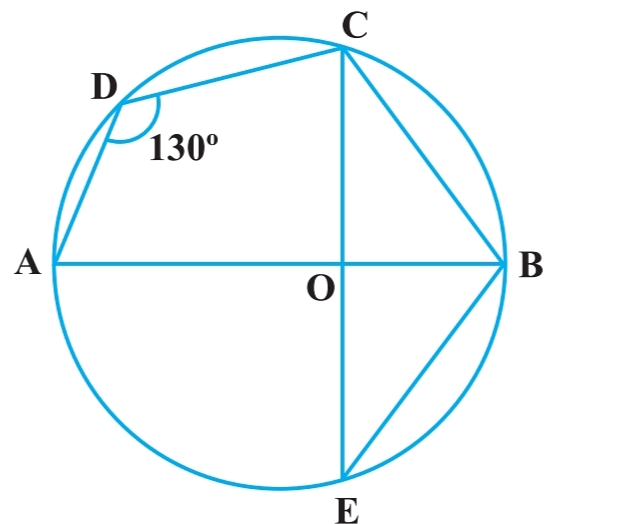
\includegraphics[width=\columnwidth]{figs/image1.jpg}
\caption{}
\label{fig:1}
\end{figure}
\item In Fig\ref{fig:2} $\angle ACB = 40\degree$. Find $\angle OAB $.
\begin{figure}[h!]
   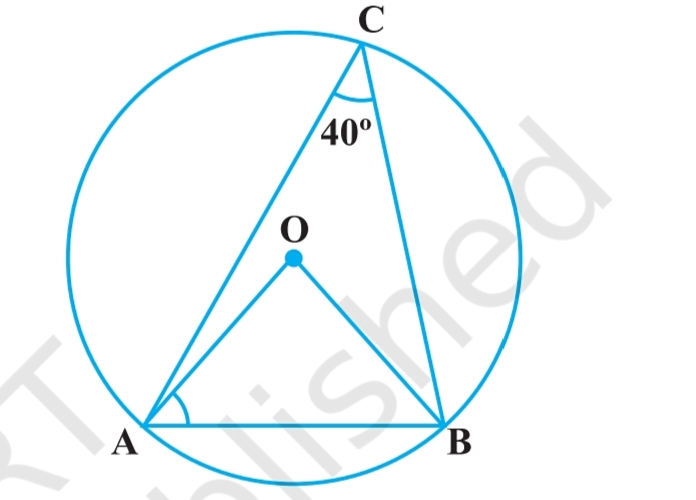
\includegraphics[width=\columnwidth]{figs/image2.jpg}
\caption{}
\label{fig:2}
\end{figure}
\item A quadrilateral ${ABCD}$ is inscrided in a circle such that $AB$ is a diameter and $\angle{ABC} = 130\degree$. Find $\angle{BAC}$.
\item Two circles with centres $\vec{O}$\text{ and }$\vec{O}\prime$ intersect at two points $\vec{A}\text{ and }\vec{B}$. A line $PQ$ is drawn parallel to $OO\prime$ through $A(or B)$ intersecting the circles at $P$ and $Q$. Prove that $PQ$=2  $OO$' .
\item In Fig\ref{fig:3} $AOB$ is a diameter of the circle and $\vec{C},\vec{D},\vec{E}$ are any three points of the semi-circle. Find the value of $\angle ACD + \angle BED$.
\begin{figure}[h!]
   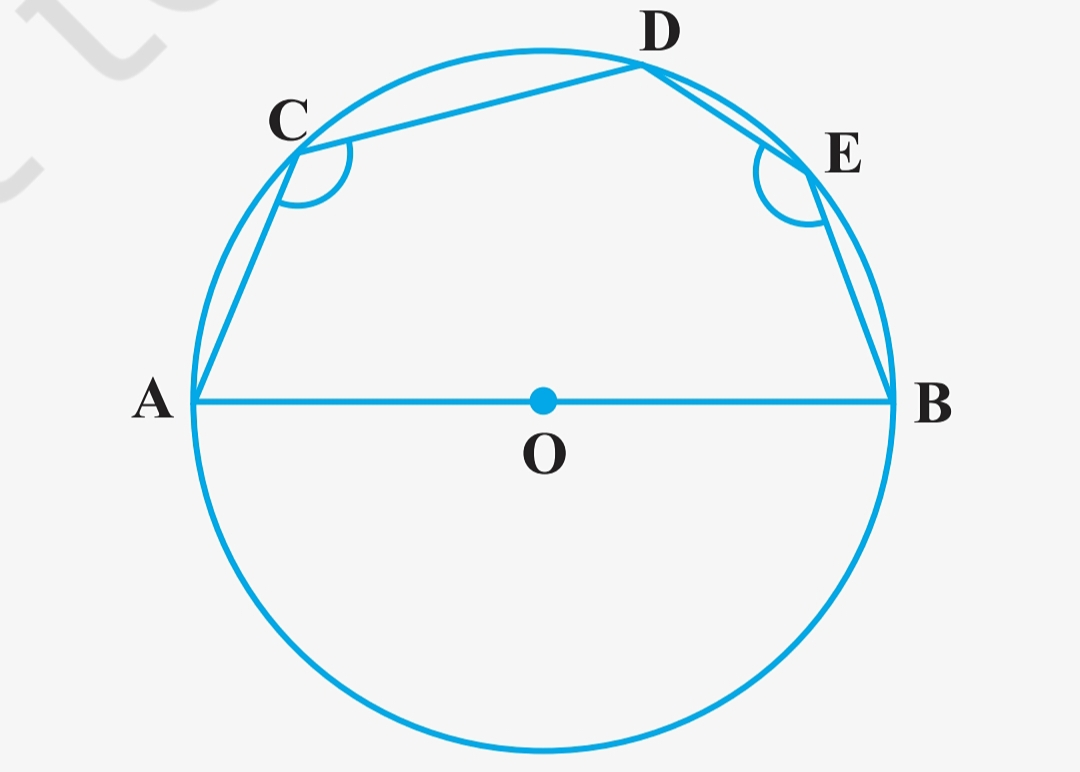
\includegraphics[width=\columnwidth]{figs/image3.jpg}
\caption{}
\label{fig:3}
\end{figure}
\item In Fig\ref{fig:4} $\angle OAB = 30\degree\text{ and }\angle OCB = 57\degree$. Find $\angle BOC\text{ and }\angle AOC$.
\begin{figure}[h!]
   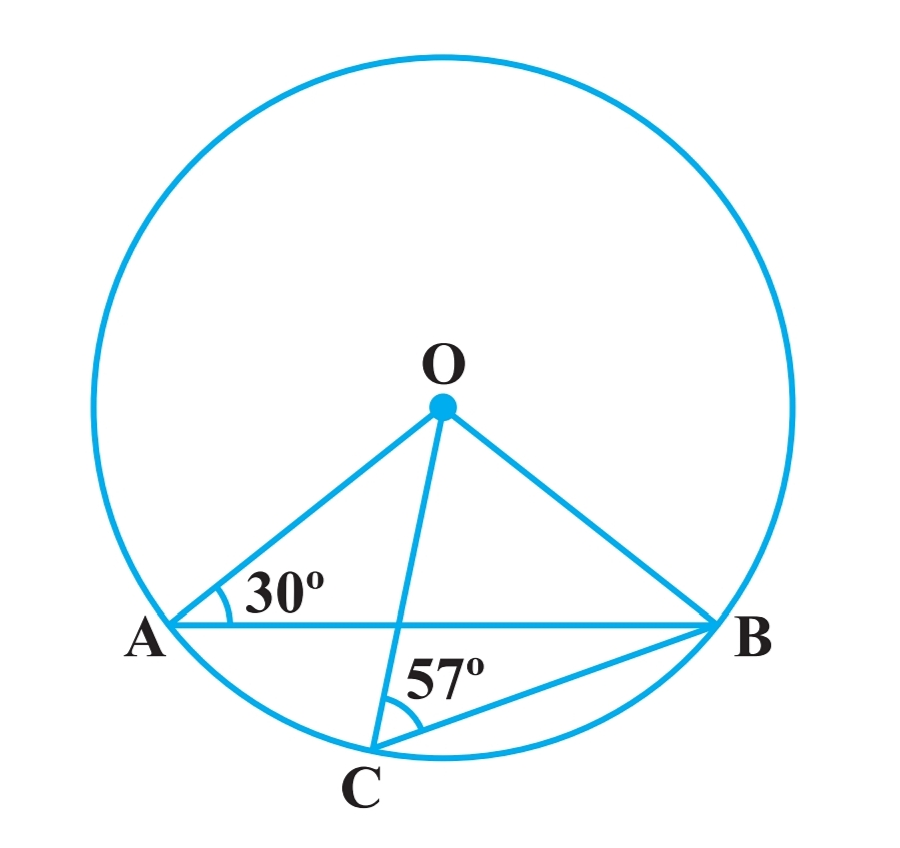
\includegraphics[width=\columnwidth]{figs/image4.jpg}
\caption{}
\label{fig:4}
\end{figure}
\end{enumerate}
\end{document}
